\documentclass[12pt]{article}
\usepackage{amsmath}
\usepackage{graphicx}
\begin{document}


\textbf{a}. Derive the trapping condition in midplane (z=0) energy coordinates for ions
in a magnetic mirror machine with mirror ratio $R\equiv B_{max}/B_{min}$ and mirror axis in
the $\hat{z}$ direction.
\vspace{3mm}

I shall assume that "midplane" refers to the center of the magnetic "potential" (minimum B)
$$R\equiv\frac{B_{max}}{B_{min}}$$
Assuming no external work, torque, and a negligible potential energy, we have that both angular momentum and kinetic energy is conserved:
$$KE=\frac{1}{2}m\vec{v}\cdot\vec{v}=const$$
$$\vec{L}=m\vec{v}\wedge\vec{r}$$
Therefore, we can take advantage of the explanation in Sect.\ref{subsecmagmirprin} to state that the velocity along the magnetic field lines can be written as:
$$v_{\parallel}^2=\frac{2}{m}(KE-\mu B)$$ 
The turning points are defined as the location where the parallel velocity vanishes, or the locations $s^*_{\pm}$ where:
$$KE=\mu B(s^*_{\pm})$$
In terms of minimum $B$ and $R$, the maximum kinetic energy that a particle can posses while still being trapped is:
$$KE=\mu B_{max}=\mu R B_{min}$$
We can derive a trapping condition in terms of $W_{\parallel0}$ and $W_{\perp0}$ via a energy balance:
$$W_{\perp0}+W_{\parallel0}=W_{\parallel0}+\mu B_0=\mu B_1$$
where $\frac{B_1}{B_0}=R$, we can rearrange to get 
$$W_{\parallel0}=\frac{W_{\perp0}}{B_0}(B_1-B_0)=W_{\perp0}(R-1)$$
And so 
$$\boxed{W_{\parallel0}\leq W_{\perp0}(R-1)}$$
Is the trapping condition
\vspace{3mm}

\noindent\textbf{b}. Sketch the trapping condition in the $W_{\perp 0}-W_{\parallel 0}$ plane, where $W_{\perp 0}$ and $W_{\parallel 0}$ are the perpendicular and parallel energies as the midplane is crossed.
\vspace{1mm}

From the previous problem, we get a straight line with a slope of $(R-1)$ (which is definitionally positive), and any particle with energy below the line, will be trapped.
\vspace{3mm}

\noindent\textbf{c}. Suppose that the magnetic field near the axis can be approximated as
$$\vec{B}= \begin{cases} 
      B_0(1+z^2/L^2)\hat{z} & z^2< c^2L^2 \\
      B_0(1+c^2)\hat{z} & z^2> c^2L^2 
   \end{cases}
$$
Show that the turning points for trapped ions obey: $z^2_T/L^2=W_{\parallel 0}/W_{\perp0}$

From part a. we know $W_{\parallel0}+W_{\perp0}=\mu B$, as well, a trapped particle must be contained in a finite region, therefore
$$W_{\parallel0}+W_{\perp0}=\mu B_0+\frac{\mu B_0 z^2}{L^2}$$
From part a. we know that the perpendicular component of the energy at the midplane is $W_{\perp0}=\mu B_0$ so the trapping condition becomes:
$$W_{\perp 0}\left(\frac{W_{\parallel0}}{W_{\perp0}}+1\right)=W_{\perp0}+\frac{W_{\perp0}z^2}{L^2}$$
$$\frac{W_{\parallel0}}{W_{\perp0}}+1=1+\frac{z^2}{L^2}$$
Therefore
$$\boxed{\frac{W_{\parallel0}}{W_{\perp0}}=\frac{z^2}{L^2}}$$
We can use a similar method to derive bounce frequency. We start with an energy balance with the left hand side NOT at the midplane, and the right hand side at one of the turning points:
$$W_{\parallel}+W_{\perp}=\mu B(z_T)$$
If we expand the magnetic field term we get
$$\frac{1}{2}mv_{\parallel}^2+\frac{\mu B_0}{L^2}z^2=\frac{\mu B_0}{L^2}z^2_T$$
We can solve for $\frac{dz}{dt}$ to find an ordinary differential equation
$$\frac{dz}{dt}=\sqrt{C-\frac{2W_{\perp 0}}{mL^2}z^2}$$
If we take a time derivative of both sides we get
$$\frac{d^2z}{dt^2}=-\frac{v_{\perp0}^2}{L^2}z$$
Therefore, the bounce frequency of a trapped particle is 
$$\omega_T=\frac{v_{\perp0}}{L}$$
By using the same method, we find that introducing a gravitational field does not change the bounce frequency.

\vspace{12mm}
Suppose now that the mirroring particles are in an axial gravitational field: $-g\hat{z}$

\noindent\textbf{d}. Write the new trapping condition in the midplane  (z=0)

With the influence of gravity, the total energy gains a term accounting for the gravitational potential: $mgh$, so the total energy is now
$$E=KE+mgh=\frac{1}{2}m(v_{\perp}^2+v_{\parallel}^2)+mgh$$
From \eqref{firstadia}, we know that $\mu=\frac{1}{2}\frac{mv_{\perp}^2}{B}$ is conserved, and therefore $\frac{1}{2}mv_{\perp}^2=\mu B$ and
$$E=\mu B +\frac{1}{2}mv_{\parallel}^2+mgh$$
and 
$$\boxed{v_{\parallel}^2=\frac{2}{m}[E-\mu B-mgz]}$$
However, it is much more useful to repeat part a:
$$W_{\parallel0}+W_{\perp0}=W_{\parallel0}+\mu B_0=\mu B_1-mgL$$
Where $L$ is the mirror machine's half length, and it was evaluated at the negative point from the mid-plane because that is where the gravitational potential is at its minimum, so particles will gather there. As well, if the particle does not turn before reaching the end of the mirror machine, it will definitely not turn, therefore, we can use $-cL$ as the minimum turning point. If we again define $R\equiv\frac{B_1}{B_0}$, the trapping condition becomes:
$$\boxed{W_{\parallel0}\leq W_{\perp0}(R-1)-cmgL}$$
We can redefine the coordinate system as $L'\equiv cL$, so the trapped B-field condition becomes:
$$B=B_0\left(1+c^2\frac{z^2}{L'^2}\right)$$
So, $R=1+c^2$ and $c^2=R-1$, so
$$B=B_0\left(1+(R-1)\frac{z^2}{L'^2}\right)$$
Note that if $R=2$ the form of $B$ is the same in either coordinate system. In this coordinate system:
$$\boxed{W_{\parallel0}\leq W_{\perp0}(R-1)-mgL'}$$
Note that 
$$L=\frac{L'}{\sqrt{R-1}}$$
Will be an important identity throughout the rest of the problem.

\vspace{3mm}

\noindent\textbf{e}. Derive the new turning points, defining the high turning point as $z_H$ and the low
turning point as $z_L$. Express $z_H$ and $z-L$ in terms of $z_T$ and $z_g$, where $z_g \equiv mgL^2
/W_{\perp 0}$.
Show that trapped particles always cross the midplane.

The turning points occur when $v_{\parallel}=0$ so $0=E-\mu B -mgz_{L/H}$, the energy is conserved, so I'll evaluate it at $z=0$, therefore:
$$\mu B+mgz=W_{\perp0}+W_{\parallel0}$$
I'll also assume that the magnetic field has the same form as in part c. such that
$$\mu B_0(1+z^2/L^2)+mgz=W_{\perp0}+W_{\parallel0}$$
Evaluating at $z=0$ and taking advantage of the first adiabatic invariant we get $\mu B_0=W_{\perp0}$ so,
$$(1+(R-1)z^2/L'^2)+\frac{mgz}{W_{\perp0}}=1+\frac{W_{\parallel0}}{W_{\perp0}}$$
rearranging, we get a quadratic equation:
$$(R-1)\frac{z^2}{L'^2}+\frac{mg}{W_{\perp0}}z-(R-1)\frac{z^2_T}{L'^2}=0$$
We can multiply through by $\frac{L'^2}{(R-1)}$ to get
$$z^2+z_gz-z_T^2=0$$
Which can be solved via the quadratic equation
$$\boxed{z_{L,H}=\frac{-z_g\pm\sqrt{z^2_g+4z_T^2}}{2}}$$ 
For the $+$ case of the quadratic equation, the root is positive because $\sqrt{z^2_g+4z^2_T}>z_g$ and thus is a positive value, and so the particle must cross the midplane.
\vspace{3mm}
 
\noindent Suppose now that the axial gravitational field is not constant, but instead increases
very slowly in time from zero at time t = 0 to a finite value g at time $t = t_f$ . (Hint: You
may find it convenient to write the parallel energy as a function of $W_{\perp 0}$, $z_H$, $z_L$ and z)
\vspace{3mm}

\noindent\textbf{f}. What is the change in the perpendicular midplane energy $W_{\perp 0}$?

We know that $\mu=\frac{W_{\perp0}}{B}$ is the first adiabatic invariant from \eqref{firstadia} so it does not vary with $g$, so 
$$\boxed{\Delta W_{\perp0}=0}$$
\vspace{3mm}

\noindent\textbf{g}. What is the change in the parallel midplane energy $W_{\parallel 0}$?

From \eqref{secondadia} we can rearrange to obtain
$$J=\sqrt{2m}\oint W_{\parallel}^{1/2}ds=const$$
Since the potential added by the variable $g$ is conservative, $E(t)$, the total energy is conserved at any fixed time $t$. So we can write $E(t)=W_{\parallel}(t)+W_{\perp}+mgz=W_{\parallel}(t)+\mu B(z)+mg(t)z=W_{\perp0}+W_{\parallel0}(t)=\mu B_0+W_{\parallel0}(t)$ so,
$$W_{\parallel0}+\mu B_0=W_{\parallel}(t)+\mu B_0(1+(R-1)z^2/L'^2)+mg(t)z$$
and
$$W_{\parallel}(t)=W_{\parallel0}(t)-(R-1)W_{\perp0}\frac{z^2}{L'^2}-mg(t)z$$
Taking into account the total loop $J$ becomes
$$J=2\sqrt{2m}\int_{z_L}^{z_H}\sqrt{W_{\parallel0}(t)-(R-1)W_{\perp0}\frac{z^2}{L'^2}-mg(t)z}dz=$$
$$\frac{2}{L'}\sqrt{2mW_{\perp0}(R-1)}\int_{z_L}^{z_H}\sqrt{\frac{W_{\parallel0}L'^2}{W_{\perp0}(R-1)}-z^2-\frac{mgL'^2}{W_{\perp0}(R-1)}}dz$$
Or
$$J=\frac{2}{L}\sqrt{2mW_{\perp0}(R-1)}\int_{z_L}^{z_H}\sqrt{z^2_T-z^2-z_gz}dz$$
If we look at the polynomial under the square root, and within the integral, and set it to zero $z_T^2-z^2-z_gz=0$, then we can multiply both sides by $-1$ to get $z^2+z_gz-z_T^2=0$, which is the equation that was solved in part h, so we know the roots, and can factor the equation
$$z^2+z_gz-z_T^2=(z-z_L)(z-z_H)$$
But we want the negative of this equation
$$z_T^2-z^2-z_gz=(z-z_L)(z_H-z)$$
So $J=\frac{2}{L'}\sqrt{2mW_{\perp0}(R-1)}\int_{z_L}^{z_H}\sqrt{(z-z_L)(z_H-z)}dz$, which can be evaluated with the given integral:
$$J=\frac{2\pi}{8L'}\sqrt{2mW_{\perp0}(R-1)}(z_H-z_L)^2$$  
At $g=0$ 
$$z_H=z_T=L'\sqrt{\frac{W_{\parallel0}}{W_{\perp0}(R-1)}}$$
$$z_L=-z_T$$
$$(z_H-z_L)^2=4L'^2\frac{W_{\parallel0}}{W_{\perp0}(R-1)}$$
and
$$J=\frac{\pi L'}{\sqrt{W_{\perp0}(R-1)}}W_{\parallel0}(0)\sqrt{2m}$$
At $g\neq 0$
$$z_H=\frac{-\frac{mgL'^2}{W_{\perp0}(R-1)}+\sqrt{\frac{m^2g^2L'^4}{W_{\perp0}^2(R-1)^2}+\frac{4W_{\parallel0}L'^2}{W_{\perp0}(R-1)}}}{2}$$
$$z_L=\frac{-\frac{mgL'^2}{W_{\perp0}(R-1)}-\sqrt{\frac{m^2g^2L'^4}{W_{\perp0}^2(R-1)^2}+\frac{4W_{\parallel0}L'^2}{W_{\perp0}(R-1)}}}{2}$$
$$(z_H-z_L)^2=\frac{m^2g^2L'^4}{W_{\perp0}^2(R-1)^2}+4L'^2\frac{W_{\parallel0}}{W_{\perp0}(R-1)}=z_g^2+4L'^2\frac{W_{\parallel0}}{W_{\perp0}(R-1)}$$
So
$$J=\frac{\pi}{4}\frac{\sqrt{2mW_{\perp0}(R-1)}}{L'}(z_g^2+4L'^2\frac{W_{\parallel0}(t_f)}{W_{\perp0}(R-1)})$$
Let's do $J(t_f)-J(0)=0=\frac{\pi z_g^2}{4L'}\sqrt{2mW_{\perp0}(R-1)}+\sqrt{\frac{2m}{W_{\perp0}(R-1)}}\pi L'\Delta W_{\parallel0}$ or
$$\boxed{\Delta W_{\parallel0}=-\frac{z_g^2W_{\perp0}(R-1)}{4L'^2}}$$
(Note: Tal Rubin gave me the solution with only math, I added explanation and worked through all the algebra explicitly, thank you Tal)
\vspace{3mm}

\noindent\textbf{h}.  In terms of the initial (t = 0) $W_{\perp 0}$ and $W_{\parallel 0}$, write down the condition for particles that are initially trapped but then detrapped. If there are any such particles, what
is the minimum $W_{\perp 0}$ and what is the minimum $W_{\parallel 0}$ (not necessarily corresponding
to the minimum $W_{\perp 0}$) that they can have?

From the previous problem
$$W_{\parallel0}(t_f)=W_{\parallel0}(0)-\frac{z_g^2W_{\perp}(R-1)}{4L'^2}$$
So, pulling from part d.
$$W_{\parallel0}(0)\leq W_{\perp0}(R-1)+\frac{m^2g^2L'^2}{4W_{\perp0}(R-1)}-mgL'$$
If we want a condition for particles to be initially trapped at $t=0$ and then detrapped by $t=t_f$ we have the double inequality:
$$W_{\perp0}(R-1)\geq W_{\parallel0}(0)\geq W_{\perp0}(R-1)+\frac{m^2g^2L'^2}{4W_{\perp0}(R-1)}-mgL'$$
This can be visualized in the following plot courtesy of Tal Rubin:

\hspace*{-2cm}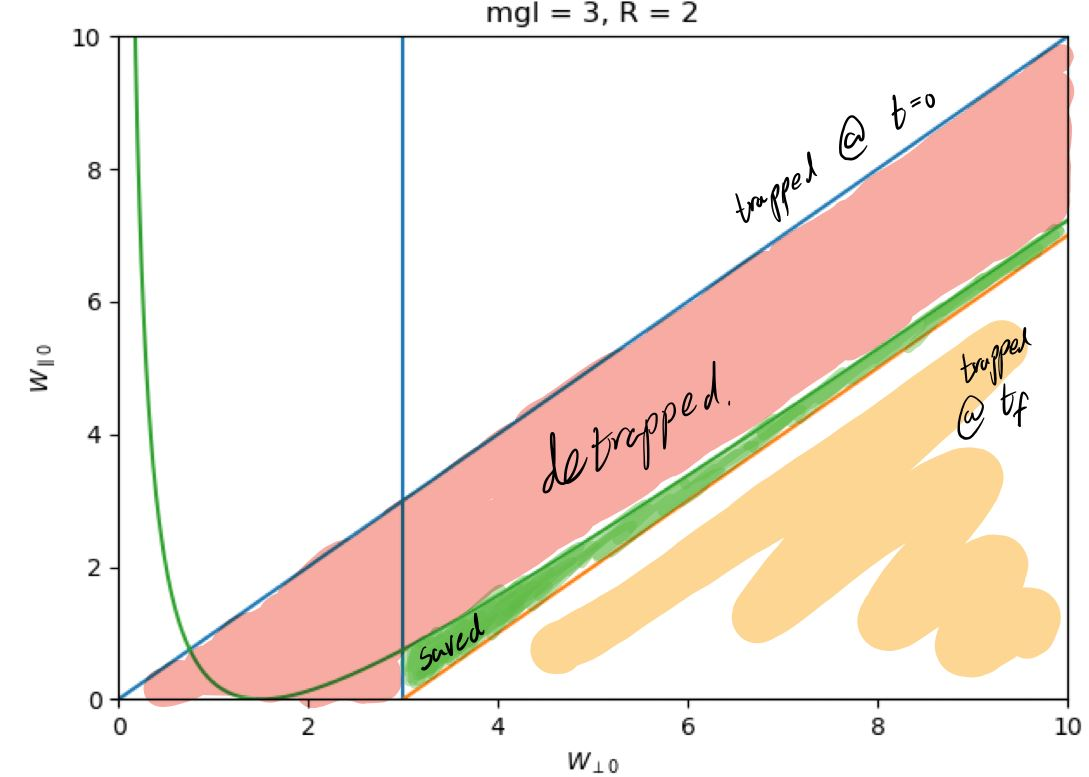
\includegraphics[scale=0.6]{GravitationalTrapping.jpg}

The minimum $W_{\perp0}$ which remains trapped is given by the zero of the orange line (the trapping condition in the $W_{\parallel0}-W_{\perp0}$ plane), it is
$$W^{min}_{\perp0}=\frac{mgL'}{R-1}$$
Then the maximum $W_{\parallel0}(0)$ at that value is:
$$W^{max}_{\parallel0}(0)=\frac{mgL'}{4}$$
We can write this in terms of c if we like:
$$W^{min}_{\perp0}=\frac{mgL}{c}$$
$$W^{max}_{\parallel0}(0)=\frac{cmgL}{4}$$
This gives a range of allowed $W_{\parallel0}$ values at the minimum $W_{\perp0}$ location which remain trapped as gravity is turned on. For detrapping, we know that the trapping condition at $t=t_f$ has shifted right by $\frac{mgL'}{R-1}$ in comparison with the condition at $t=0$ so anything to the left of $W_{\perp0}=\frac{mgL'}{R-1}$ will be detrapped, there is no such condition for $W_{\parallel0}(0)$ so we are free to set it to zero, so:
$$\boxed{W^{min}_{\perp0}=0}$$
$$\boxed{W^{min}_{\parallel0}(0)=0}$$
In other words: The question asks for the minimum values of $W_{\parallel0}$ and $W_{\perp0}$ which are initially trapped and then detrapped. The minimum values that can be trapped initially are 0,0 since it satisfies the trapping condition without gravity. When gravity is turned on the trapping condition moves the the right by $\frac{mgL’}{R-1}$ and hence detraps anything to the left of that, this includes the point 0,0. Since 0,0 is the minimum value initially trapped and it is subsequently detrapped, it must be the minimum value initially trapped and then detrapped.
\vspace{3mm}

\noindent\textbf{i}. Suppose instead the axial gravitational field starts off at a finite value g at time
t = 0, and then decreases very slowly in time to zero at time $t=t_f$. In terms of the
initial (t = 0) $W_{\perp 0}$ and $W_{\parallel 0}$, write down the condition for particles that are initially
trapped but then detrapped. If there are any such particles, what is the minimum
$W_{\perp 0}$ and what is the minimum $W_{\parallel}$ (not necessarily corresponding to the minimum
$W_{\perp 0}$) that they can have?

Since there is no additional additional potential in this problem, it is just the reverse of what was done above. meaning that instead of having the trapping condition go from a form of $W_{\parallel0}=x$ to one of the form $W_{\parallel0}=x-mgL$ we are going from $W_{\parallel0}=x-mgL$ to $W_{\parallel0}=x$, which is a shift to the left, and encloses more space, so there cannot be any trapped particles that are detrapped. (Equivalent of shifting from the orange line to the blue line above, no particles are lost)

\vspace{2mm}

Hint: You may wish to use the integral:
$$\int^b_a[(s-a)(b-s)]^{1/2}ds=\frac{\pi}{8}(b-a)^2$$
\end{document}